\documentclass[a4paper]{article}

\usepackage[english]{babel}
\usepackage[margin=1in]{geometry}
\usepackage[utf8]{inputenc}
\usepackage{amsmath}
\usepackage{graphicx}
\usepackage[colorinlistoftodos]{todonotes}

\usepackage{outlines}
\usepackage{enumitem}
\setenumerate[1]{label=\Roman*.}
\setenumerate[2]{label=\Alph*.}
\setenumerate[3]{label=\roman*.}
\setenumerate[4]{label=\alph*.}

\title{Humboldt Outline}

\author{Jospeh Christesen}

\date{\today}

\begin{document}
\maketitle

\begin{abstract}
\noindent
\begin{enumerate}
\item The current state of research should first be briefly described and underpinned by approximately five relevant publications from the research area. (one page max)  

\item The outline should focus on a clear description of the questions you intend to address in your research, their originality and significance for the advancement of the research field. (approx. two pages) 

\item Furthermore, the academic methods to be used to achieve these goals should be clearly described. (approx. two pages)

\item A comprehensive bibliography and a detailed time plan are not required. 

\item The research outline should comprise approximately five pages in total. Should you significantly exceed this length, you may be asked to cut it down to approximately five pages.

\item For the purposes of evaluation it must be clearly demonstrated that you yourself have drawn up the main contents independently and agreed them beforehand with your host. Any contents contributed by the host institute must be attributed accordingly.
\end{enumerate}
\end{abstract}

\section{Quantum Memory Storage}

\begin{outline}[enumerate]
\1 \textbf{Background}
	\2 Storage of quantum states is important for applications in quantum communication and distributed quantum computing
    \2 Neutral atoms in a cavity provide a good way for achieving quantum storage
    	\3 Long coherence times
        \3 Good coupling to a well defined photon mode
    \2 There have been several techniques implemented for quantum storage with neutral atoms
    	\3 Specht 2011
        	\4 Efficiency of 9.3 $\pm$ 1\%
            \4 No herald
        \3 Kalb 2015
        	\4 Efficiency of 25\%
            \4 Heralding of the transfer
            \4 Needs to have optimal mode matching with the cavity otherwise the photon won't interact with the atom and will reflect off of the mirror
    \2 I propose here to use the Specht scheme in a fiber-based cavity  with a crossed cavity geometry
    	\3 This will enable a passive heralding scheme which will increase the efficiency of the Specht scheme
        \3 It will also eliminate the problems with mode matching from the Kalb system
        
    
\1 \textbf{Questions to be Addressed, Originality, and Significance for Advancement in Field}


\1 \textbf{Academic methods used to achieve these goals}
    
\end{outline}

% \section{Quantum Repeater}

% \begin{outline}[enumerate]
% \1 \textbf{Background}
% 	\2 Quantum communication is an important new technology that can be used for testing fundamental problems in physics (e.g. Loophole free Bell-test), creating secure networks (e.g. quantum cryptography), and distributed quantum computing.
%     	\3 A problem is the natural losses that occur in transmission of these quantum states either through fibers or free space propagation.
%     	\3 Therefore, for transmission of quantum states to be achievable over long distances, a quantum repeater needs to be developed. The ideal system would be able to couple directly into already existing fiber-optic cables which already exhibit low loss at 1.3 $\mu$m and 1.5 $\mu$m.
% 	\2 Several technologies have been researched as possible avenues to create a quantum repeater including  atomic ensembles, single neutral atoms and ions, nitrogen vacancy centers, quantum dots, and ion-doped solids.
%     	\3 Single neutral atoms are a promising candidate as they can be isolated from the environment and provide long coherence times.
%         \3 Several parts of the quantum repeater have already been demonstrated independently. However, the schemes involve conversion of the photon at telecom wavelengths to be converted into a near-IR photon which decreases the efficiency of the repeater scheme.
% 	\2 Therefore, we propose a scheme which only uses photons at telecom wavelengths by using a novel fiber-based optical cavity design in which the neutral atom resides in two orthogonal optical cavities. 
% \1 \textbf{Schematic of repeater design}

% \1 \textbf{Fiber-based Crossed-Cavity Design}
    
% \end{outline}



% Your introduction goes here! Some examples of commonly used commands and features are listed below, to help you get started. If you have a question, please use the help menu (``?'') on the top bar to search for help or ask us a question.

% \section{Some \LaTeX{} Examples}
% \label{sec:examples}

% \subsection{How to Leave Comments}

% Comments can be added to the margins of the document using the \todo{Here's a comment in the margin!} todo command, as shown in the example on the right. You can also add inline comments:

% \todo[inline, color=green!40]{This is an inline comment.}

% \subsection{How to Include Figures}

% First you have to upload the image file (JPEG, PNG or PDF) from your computer to Overleaf using the upload link the project menu. Then use the \verb|\includegraphics| command to include it in your document. Use the figure environment and the caption command to add a number and a caption to your figure. See the code for Figure \ref{fig:frog} in this section for an example.

% \begin{figure}
% \centering
% 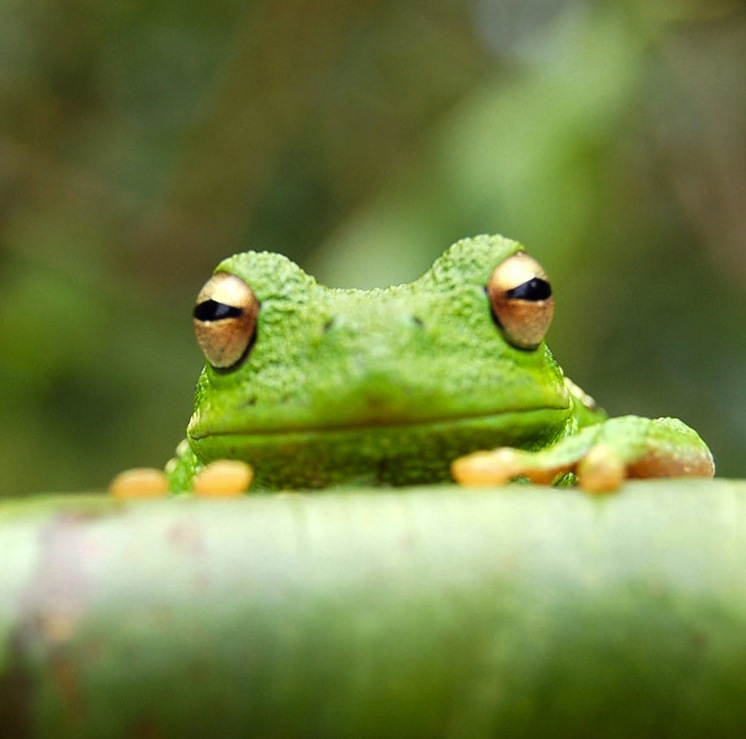
\includegraphics[width=0.3\textwidth]{frog.jpg}
% \caption{\label{fig:frog}This frog was uploaded to Overleaf via the project menu.}
% \end{figure}

% \subsection{How to Make Tables}

% Use the table and tabular commands for basic tables --- see Table~\ref{tab:widgets}, for example.

% \begin{table}
% \centering
% \begin{tabular}{l|r}
% Item & Quantity \\\hline
% Widgets & 42 \\
% Gadgets & 13
% \end{tabular}
% \caption{\label{tab:widgets}An example table.}
% \end{table}

% \subsection{How to Write Mathematics}

% \LaTeX{} is great at typesetting mathematics. Let $X_1, X_2, \ldots, X_n$ be a sequence of independent and identically distributed random variables with $\text{E}[X_i] = \mu$ and $\text{Var}[X_i] = \sigma^2 < \infty$, and let
% $$S_n = \frac{X_1 + X_2 + \cdots + X_n}{n}
%       = \frac{1}{n}\sum_{i}^{n} X_i$$
% denote their mean. Then as $n$ approaches infinity, the random variables $\sqrt{n}(S_n - \mu)$ converge in distribution to a normal $\mathcal{N}(0, \sigma^2)$.

% \subsection{How to Make Sections and Subsections}

% Use section and subsection commands to organize your document. \LaTeX{} handles all the formatting and numbering automatically. Use ref and label commands for cross-references.

% \subsection{How to Make Lists}

% You can make lists with automatic numbering \dots

% \begin{enumerate}
% \item Like this,
% \item and like this.
% \end{enumerate}
% \dots or bullet points \dots
% \begin{itemize}
% \item Like this,
% \item and like this.
% \end{itemize}
% \dots or with words and descriptions \dots
% \begin{description}
% \item[Word] Definition
% \item[Concept] Explanation
% \item[Idea] Text
% \end{description}

% We hope you find Overleaf useful, and please let us know if you have any feedback using the help menu above.

\end{document}